%%%%%%%%%%%%%%%%%%%%%%%%%%%%%%%%%%%%%%%%%
% Programming/Coding Assignment
% LaTeX Template
%
% This template has been downloaded from:
% http://www.latextemplates.com
%
% Original author:
% Ted Pavlic (http://www.tedpavlic.com)
%
% Note:
% The \lipsum[#] commands throughout this template generate dummy text
% to fill the template out. These commands should all be removed when 
% writing assignment content.
%
% This template uses a Perl script as an example snippet of code, most other
% languages are also usable. Configure them in the "CODE INCLUSION 
% CONFIGURATION" section.
%
%%%%%%%%%%%%%%%%%%%%%%%%%%%%%%%%%%%%%%%%%

%----------------------------------------------------------------------------------------
%	PACKAGES AND OTHER DOCUMENT CONFIGURATIONS
%----------------------------------------------------------------------------------------

\documentclass{article}
\usepackage{fancyhdr} % Required for custom headers
\usepackage{lastpage} % Required to determine the last page for the footer
\usepackage{extramarks} % Required for headers and footers
\usepackage[usenames,dvipsnames]{color} % Required for custom colors
\usepackage{graphicx} % Required to insert images
\usepackage{caption}
\usepackage{listings} % Required for insertion of code
\usepackage{courier} % Required for the courier font
\usepackage{lipsum} % Used for inserting dummy 'Lorem ipsum' text into the template
\usepackage[colorlinks=true,linkcolor=black,anchorcolor=black,citecolor=black,menucolor=black,runcolor=black,urlcolor=black,bookmarks=true]{hyperref}
\usepackage[table,svgnames]{xcolor}
\usepackage{tabularx}
\usepackage{booktabs}
\usepackage{natbib}
\usepackage{pdfpages}
\usepackage[T1]{fontenc}
\usepackage{amsmath}


% Margins
\topmargin=-0.45in
\evensidemargin=0in
\oddsidemargin=0in
\textwidth=6.5in
\textheight=9.0in
\headsep=0.25in

\linespread{1.1} % Line spacing

% Set up the header and footer
\pagestyle{fancy}
\lhead{\hmwkAuthorName} % Top left header
\chead{\hmwkClass\ (\hmwkClassInstructor\ \hmwkClassTime): \hmwkTitle} % Top center head
\rhead{\firstxmark} % Top right header
\lfoot{\lastxmark} % Bottom left footer
\cfoot{} % Bottom center footer
\rfoot{Page\ \thepage\ of\ \protect\pageref{LastPage}} % Bottom right footer
\renewcommand\headrulewidth{0.4pt} % Size of the header rule
\renewcommand\footrulewidth{0.4pt} % Size of the footer rule

\setlength\parindent{0pt} % Removes all indentation from paragraphs

%----------------------------------------------------------------------------------------
%	CODE INCLUSION CONFIGURATION
%----------------------------------------------------------------------------------------

\definecolor{MyDarkGreen}{rgb}{0.0,0.4,0.0} % This is the color used for comments
\lstloadlanguages{Perl} % Load Perl syntax for listings, for a list of other languages supported see: ftp://ftp.tex.ac.uk/tex-archive/macros/latex/contrib/listings/listings.pdf
\lstset{language=Perl, % Use Perl in this example
        frame=single, % Single frame around code
        basicstyle=\small\ttfamily, % Use small true type font
        keywordstyle=[1]\color{Blue}\bf, % Perl functions bold and blue
        keywordstyle=[2]\color{Purple}, % Perl function arguments purple
        keywordstyle=[3]\color{Blue}\underbar, % Custom functions underlined and blue
        identifierstyle=, % Nothing special about identifiers                                         
        commentstyle=\usefont{T1}{pcr}{m}{sl}\color{MyDarkGreen}\small, % Comments small dark green courier font
        stringstyle=\color{Purple}, % Strings are purple
        showstringspaces=false, % Don't put marks in string spaces
        tabsize=5, % 5 spaces per tab
        %
        % Put standard Perl functions not included in the default language here
        morekeywords={rand},
        %
        % Put Perl function parameters here
        morekeywords=[2]{on, off, interp},
        %
        % Put user defined functions here
        morekeywords=[3]{test},
       	%
        morecomment=[l][\color{Blue}]{...}, % Line continuation (...) like blue comment
        numbers=left, % Line numbers on left
        firstnumber=1, % Line numbers start with line 1
        numberstyle=\tiny\color{Blue}, % Line numbers are blue and small
        stepnumber=5 % Line numbers go in steps of 5
}

% Creates a new command to include a perl script, the first parameter is the filename of the script (without .pl), the second parameter is the caption




%----------------------------------------------------------------------------------------
%	DOCUMENT STRUCTURE COMMANDS
%	Skip this unless you know what you're doing
%----------------------------------------------------------------------------------------

% Header and footer for when a page split occurs within a problem environment
\newcommand{\enterProblemHeader}[1]{
\nobreak\extramarks{#1}{#1 continued on next page\ldots}\nobreak
\nobreak\extramarks{#1 (continued)}{#1 continued on next page\ldots}\nobreak
}

% Header and footer for when a page split occurs between problem environments
\newcommand{\exitProblemHeader}[1]{
\nobreak\extramarks{#1 (continued)}{#1 continued on next page\ldots}\nobreak
\nobreak\extramarks{#1}{}\nobreak
}

\setcounter{secnumdepth}{0} % Removes default section numbers
\newcounter{homeworkProblemCounter} % Creates a counter to keep track of the number of problems

\newcommand{\homeworkProblemName}{}
\newenvironment{homeworkProblem}[1][Problem \arabic{homeworkProblemCounter}]{ % Makes a new environment called homeworkProblem which takes 1 argument (custom name) but the default is "Problem #"
\stepcounter{homeworkProblemCounter} % Increase counter for number of problems
\renewcommand{\homeworkProblemName}{#1} % Assign \homeworkProblemName the name of the problem
\section{\homeworkProblemName} % Make a section in the document with the custom problem count
\enterProblemHeader{\homeworkProblemName} % Header and footer within the environment
}{
\exitProblemHeader{\homeworkProblemName} % Header and footer after the environment
}

\newcommand{\problemAnswer}[1]{ % Defines the problem answer command with the content as the only argument
\noindent\framebox[\columnwidth][c]{\begin{minipage}{0.98\columnwidth}#1\end{minipage}} % Makes the box around the problem answer and puts the content inside
}

\newcommand{\homeworkSectionName}{}
\newenvironment{homeworkSection}[1]{ % New environment for sections within homework problems, takes 1 argument - the name of the section
\renewcommand{\homeworkSectionName}{#1} % Assign \homeworkSectionName to the name of the section from the environment argument
\subsection{\homeworkSectionName} % Make a subsection with the custom name of the subsection
\enterProblemHeader{\homeworkProblemName\ [\homeworkSectionName]} % Header and footer within the environment
}{
\enterProblemHeader{\homeworkProblemName} % Header and footer after the environment
}

%----------------------------------------------------------------------------------------
%	NAME AND CLASS SECTION
%----------------------------------------------------------------------------------------

\newcommand{\hmwkTitle}{A4} % Assignment title
\newcommand{\hmwkDueDate}{Monday,\ December\ 4,\ 2017} % Due date
\newcommand{\hmwkClass}{\ INTRO. TO INFO RETRIEVAL:\ CS 734} % Course/class
\newcommand{\hmwkClassTime}{} % Class/lecture time
\newcommand{\hmwkClassInstructor}{Dr. Nelson} % Teacher/lecturer
\newcommand{\hmwkAuthorName}{Udochukwu Nweke} % Your name

%----------------------------------------------------------------------------------------
%	TITLE PAGE
%----------------------------------------------------------------------------------------

\title{
\vspace{2in}
\textmd{\textbf{\hmwkClass:\ \hmwkTitle}}\\
\normalsize\vspace{0.1in}\small{Due\ on\ \hmwkDueDate}\\
\vspace{0.1in}\large{\textit{\hmwkClassInstructor\ \hmwkClassTime}}
\vspace{3in}
}

\author{\textbf{\hmwkAuthorName}}
\date{} % Insert date here if you want it to appear below your name

%----------------------------------------------------------------------------------------

\begin{document}

\maketitle

%----------------------------------------------------------------------------------------
%	TABLE OF CONTENTS
%----------------------------------------------------------------------------------------

%\setcounter{tocdepth}{1} % Uncomment this line if you don't want subsections listed in the ToC

\newpage
\tableofcontents
\newpage

%----------------------------------------------------------------------------------------
%	PROBLEM 1
%----------------------------------------------------------------------------------------

% To have just one problem per page, simply put a \clearpage after each problem

\begin{homeworkProblem}


9.10. Nearest neighbor clusters are not symmetric, in the sense that if instance A is one of instance B's nearest neighbors, the reverse is not necessarily true. Explain how this can happen with a diagram.\\

\textbf{Solution 1:}\\

Figure 1 shows that  nearest neighbors are not symmetric. It can be seen that although A is B's nearest neighbor because A has the closest distance to B compared to C and D, the reverse is not the case here because B is not the closest distance to A. E is  A's nearest neighbor because E has the smallest distance to A. This explains how nearest neighbors are not symmetric. 

\begin{figure}
 \centering
  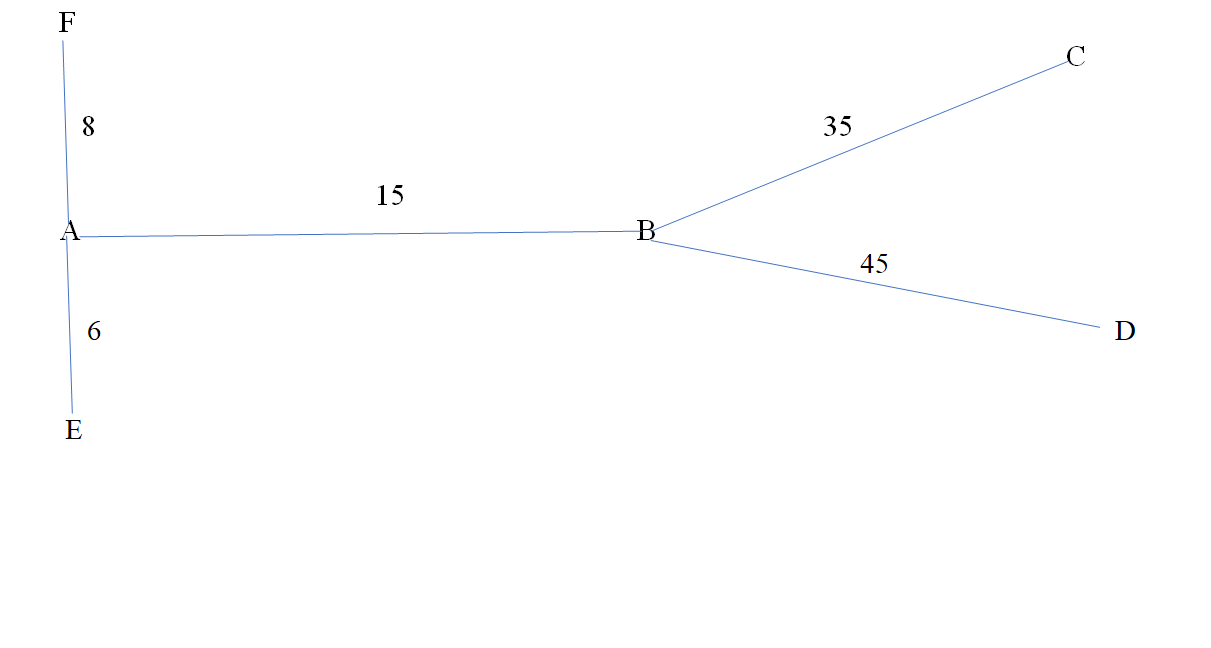
\includegraphics[width=0.5\textwidth]{unsymetrcKnn.png}
 \caption{Asymetric Nearest neighbor}
 \end{figure}


 \end{homeworkProblem}
%----------------------------------------------------------------------------------------
% PROBLEM 2
%----------------------------------------------------------------------------------------


\begin{homeworkProblem}

9.11. The K nearest neighbors of a document could be represented by links to those documents. Describe two ways this representation could be used in a search application.\\


\textbf{Solution 2:}\\

 K nearest neighbors of a document  could be represented by links to those documents. This means that document will be linked to similar documents. These similar documents are considered the nearest neighbor of the document.  K-NN can be used in search application where a user's task is to find items that are ``similar to a particular item''. This is referred to as K-NN search.
Similarity is measured by creating a vector representation of the documents links, then we use a distance metric (Euclidean distance) to compare the vectors, or cosine similarity.\\

Examples of K-NN search:\\

\textbf{Concept Search}: In concept search, a user searches documents that contain similar topics. Concept search is found in several e-Discovery software packages, which are used to help organizations find all  the e-mails, contracts, etc. that are relevanant to the organization.\\

\textbf{Recommender Systems}:Another use of K-NN search is recommender systems.  If a user likes a particular item, a similar item can be recommended to them.  K-NN search helps find similar items. If similar users liked two different items, it is possible that the items are similar.
This is used in recommending products, recomemending advertisements to display to a user, etc.


\end{homeworkProblem}

%----------------------------------------------------------------------------------------
% PROBLEM 3
%----------------------------------------------------------------------------------------


\begin{homeworkProblem}


9.8. Cluster the following set of two-dimensional instances into three clusters using
each of the five agglomerative clustering methods:\\
(-4, -2), (-3, -2), (-2, -2), (-1, -2), (1, -1), (1, 1), (2, 3), (3, 2), (3, 4), (4, 3)\\
Discuss the differences in the clusters across methods. Which methods produce
the same clusters? How do these clusters compare to how you would manually
cluster the points?\\

\textbf{Solution 3:}\\

\lstinputlisting[caption=Agglomerative Clustering Code Snippet, language=python]{9.8.py}
\begin{enumerate}
\item Agglomerative clustering is a type of hierarchical clustering.  In agglomerative clustering, each data point is defined to be a cluster, and existing clusters are combined at each step. There are for different methods for achieving these steps and they are:
\item \textbf{Single Linkage}: In this method of clustering, the distance between two clusters is defined to be the minimum distance between any single data point in cluster A and any single data point in cluster B. At each stage in the process, the two clusters that have the smallest single linkage distance is combined.
\item \textbf{Complete Linkage}: In complete linkage, the distance between two clusters is defined to be the maximum distance between any single data point in the first cluster and any single data point in the second cluster. At each step, the two clusters that have the smallest complete linkage distance is combined.
\item \textbf{Average Linkage}: In this method of clustering, the distance between two clusters is defined to be the average distance between data points in the first cluster and the data points in the second cluster. At each step, the two clusters that have the smallest average link distance is combined.
\item \textbf{Centroid Approach}: In this approach, the distance between two clusters is defined as the distance between two mean vectors of the clusters. At each step, the two clusters that have the smallest centroid distance is combined.
\item \textbf{Ward's Approach}: This approach is not based on distances of two clusters like the previous agglomerative method. Wards is based on the statistical property of variation. The variance of a set of numbers measures how spread out the numbers are. 
\end{enumerate}

Figure \ref{fig: clusteringmthds} shows how the different agglomerative clustering methods are represented.\\

I used \textit{clustering()} in Listing 1 to cluster the given set of two-dimensional instances into three clusters using the five agglomerative clustering method I have explained. \\

All linkages resulted in the same clustering when K=3. This gave me some concern. For some time, I thought I was doing something wrong or there was something wrong with the algorithm. When I changed the number of K, the clustering was different. 
For K= 3, all 5 methods gave the same clustering and the case is different when K is not 3. K= 2 gave the same clustering for average method, ward method, and complete method. The result of the clustering can be seen in Figures \ref{fig: singlelinkage}, \ref{fig: completelinkage}, \ref{fig: averagelinkage}, \ref{fig: centroidlinkage}, and \ref{fig: wardlinkage} respectively.\\

For manual clustering, I used \textit{plotOriginalPoints()} in Listing 1 to manually cluster the given set of two-dimensional instances. The result is in Figure \ref{fig: originalman}. The result shows that the algorithm did well K= 3 and K= 2 clusterings showed similar clustersing pattern with the manual clustering.\\

My manual clustering of the given set of the two-dimensional instances into three clusters will be as follows:\\
Cluster 1: Point 1,2,3,4\\
Cluster 2: Point 5,6\\
Cluster 3: point 7,8,9,10


\begin{figure}
 \centering
  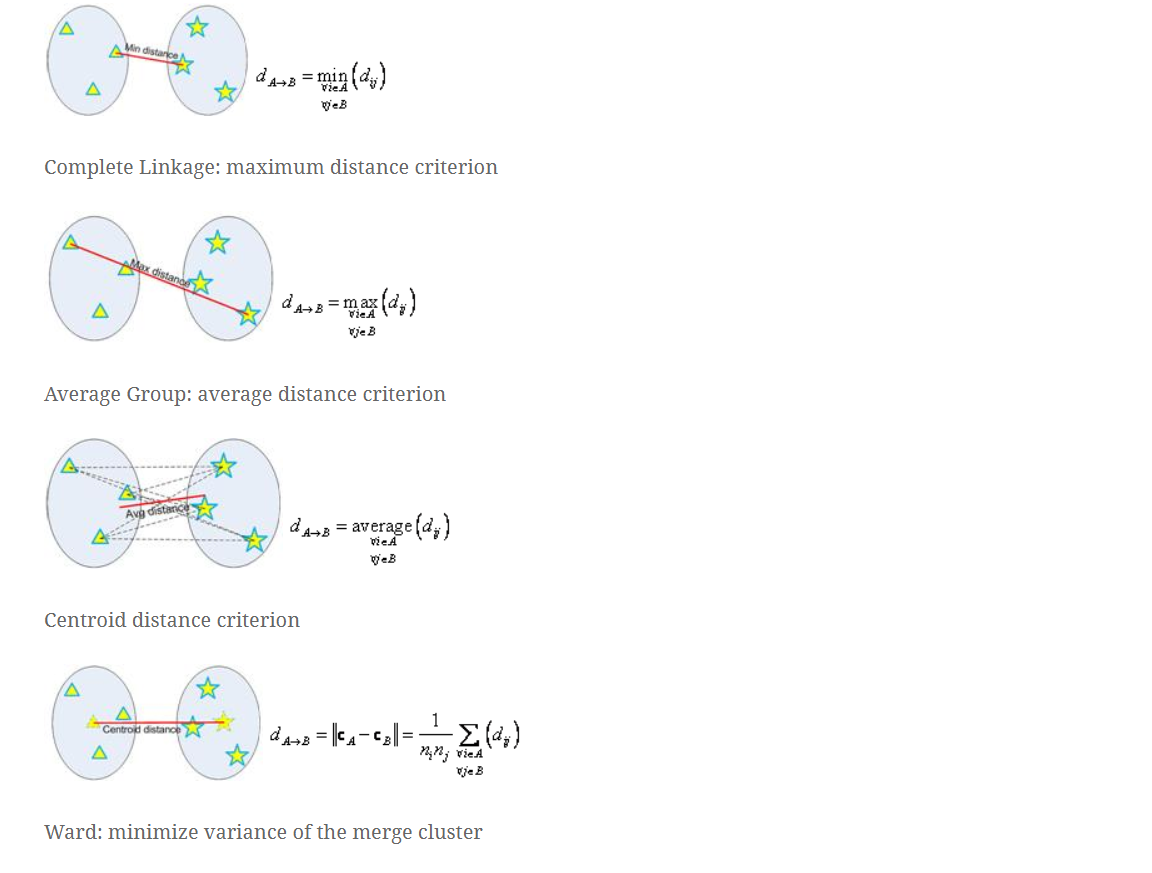
\includegraphics[width=0.5\textwidth]{Agclustering.png}
 \caption{Agglomerative Clustering Methods}
 \label{fig: clusteringmthds}
 \end{figure}



\begin{figure}
 \centering
  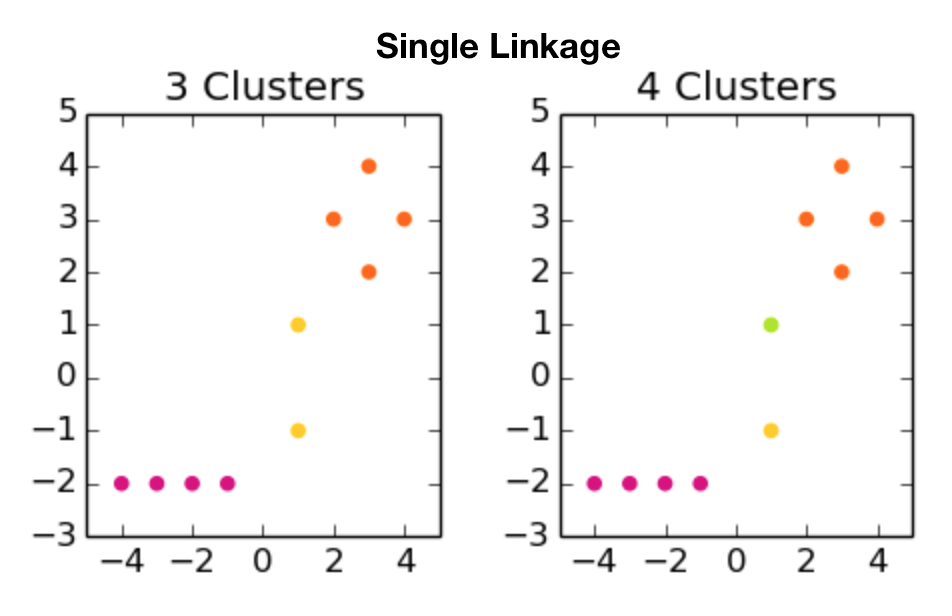
\includegraphics[width=0.5\textwidth]{single-3-4.png}
 \caption{Single Linkage}
 \label{fig: singlelinkage}
 \end{figure}

\begin{figure}
 \centering
  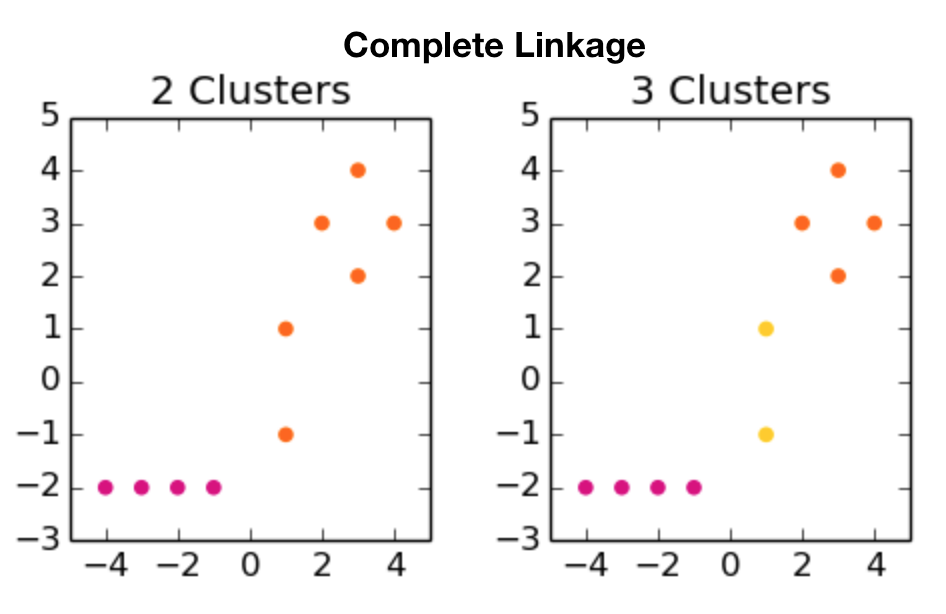
\includegraphics[width=0.5\textwidth]{complete-2-3.png}
 \caption{Complete Linkage}
 \label{fig: completelinkage}
 \end{figure}

\begin{figure}
 \centering
  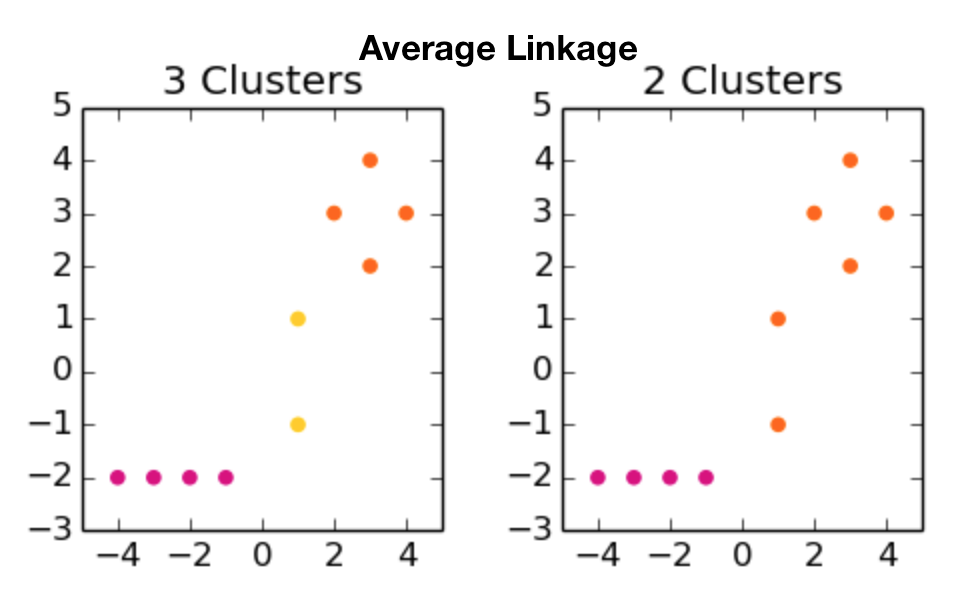
\includegraphics[width=0.5\textwidth]{average-2-3.png}
 \caption{average Linkage}
 \label{fig: averagelinkage}
 \end{figure}

 \begin{figure}
 \centering
  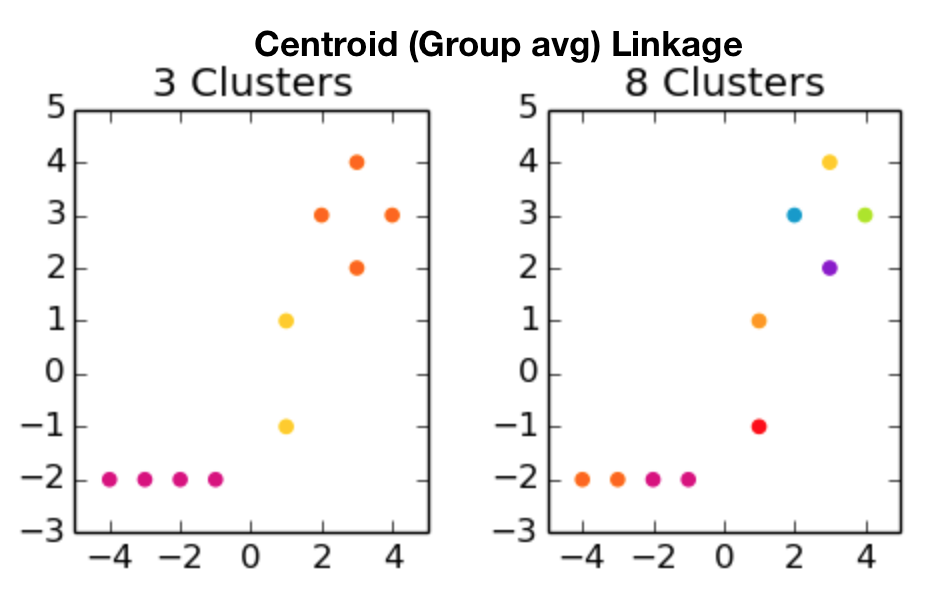
\includegraphics[width=0.5\textwidth]{centroid-3-8.png}
 \caption{Centroid Linkage}
 \label{fig: centroidlinkage}
 \end{figure}

 \begin{figure}
 \centering
  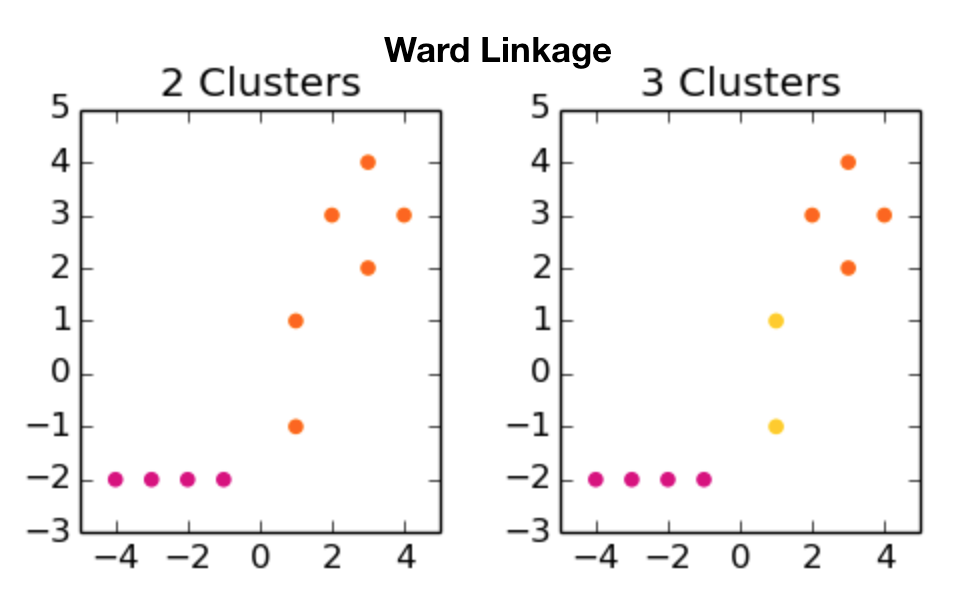
\includegraphics[width=0.5\textwidth]{ward-2-3.png}
 \caption{Ward Linkage}
 \label{fig: wardlinkage}
 \end{figure}

\begin{figure}
 \centering
  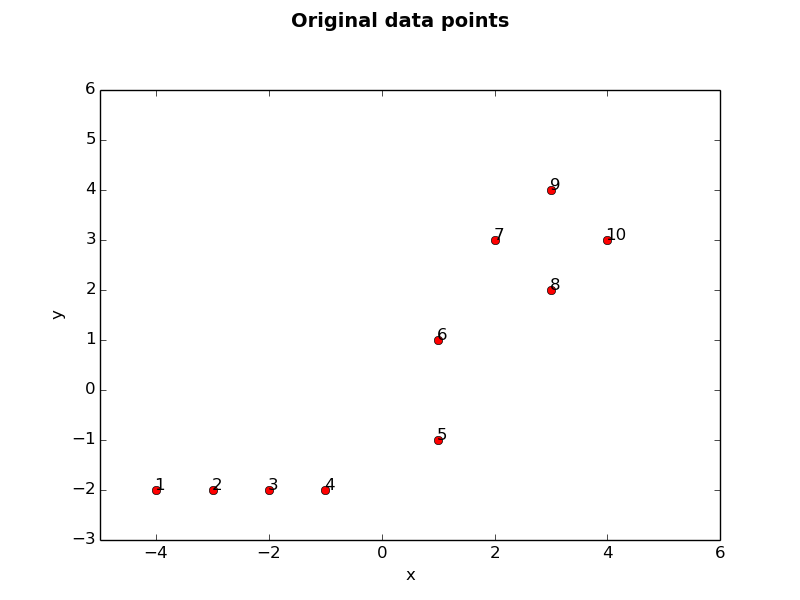
\includegraphics[width=0.5\textwidth]{originalPoints.png}
 \caption{Manual Clustering}
 \label{fig: originalman}
 \end{figure}






\end{homeworkProblem}

%----------------------------------------------------------------------------------------
% PROBLEM 4
%----------------------------------------------------------------------------------------

\begin{homeworkProblem}

9.6. Compare the accuracy of a one versus all SVM classifier and a one versus
one SVM classifier on a multiclass classification data set. Discuss any differences
observed in terms of the efficiency and effectiveness of the two approaches.\\

\textbf{Solution 4:}\\


 \begin{figure}
 \centering
  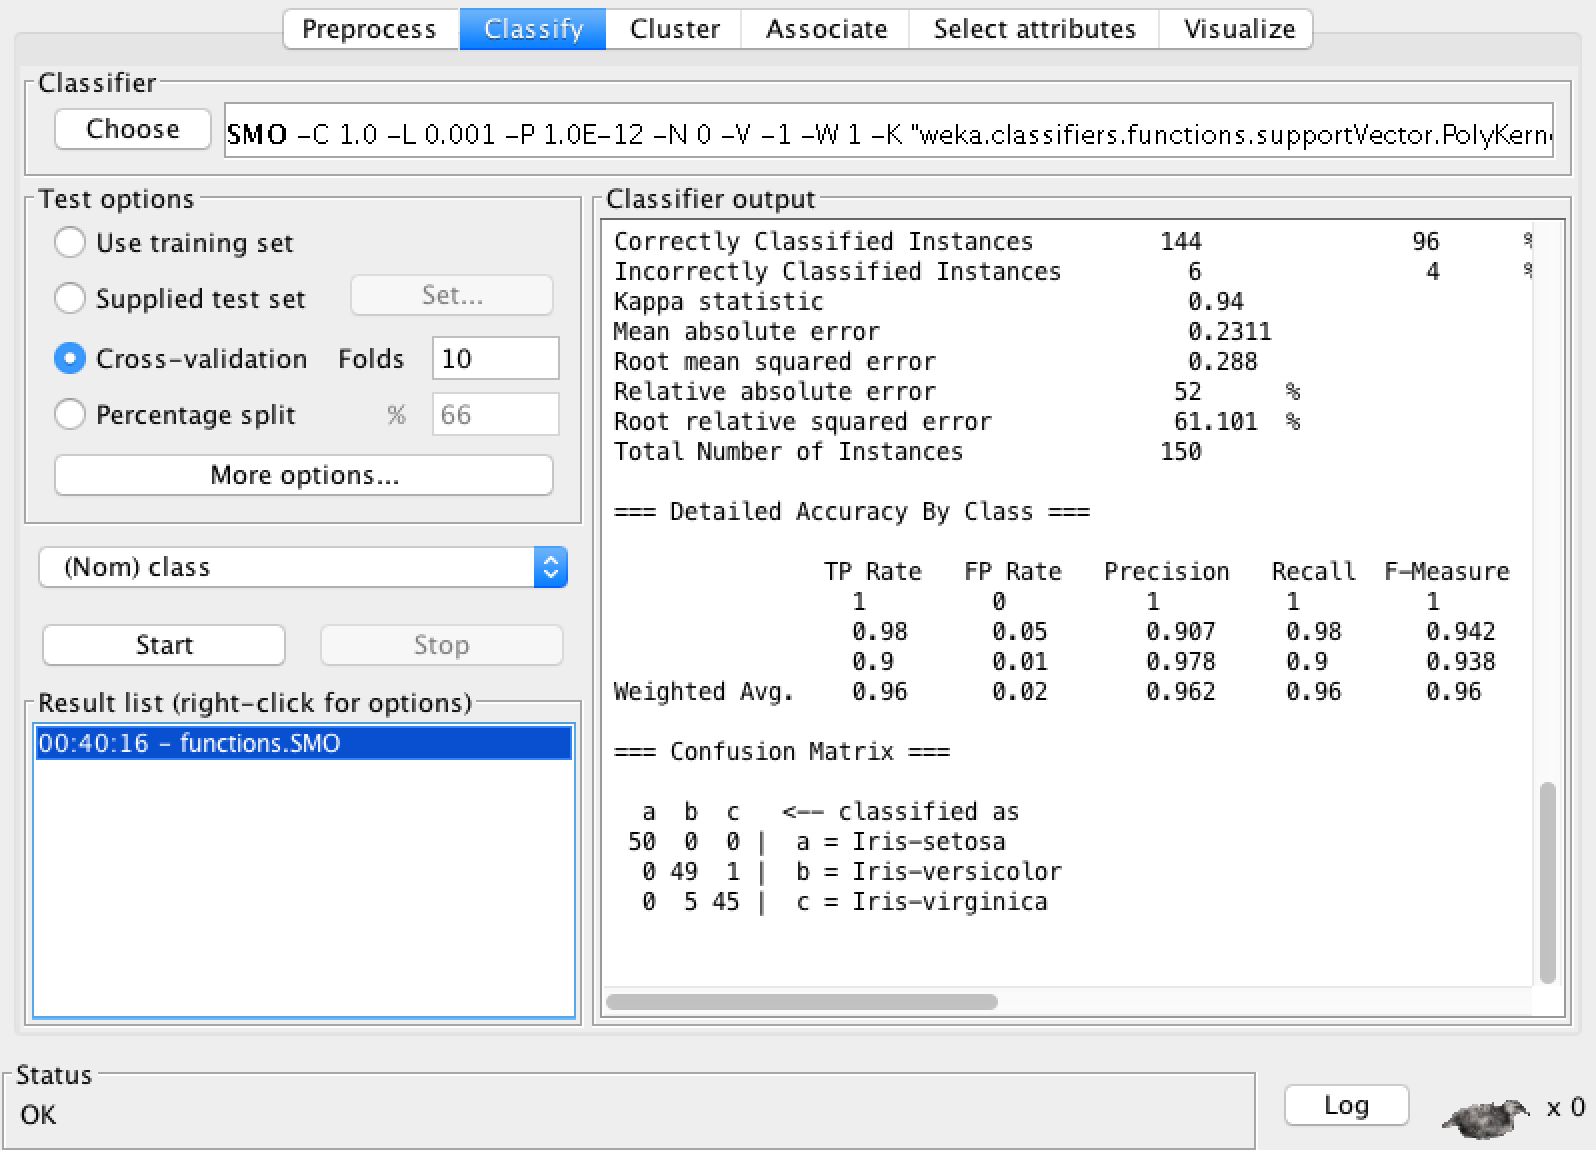
\includegraphics[width=0.5\textwidth]{wekaOneVsOneResult.png}
 \caption{oneVsOne SVM Classifier result}
 \label{fig: onevsone}
 \end{figure}

 \begin{figure}
 \centering
  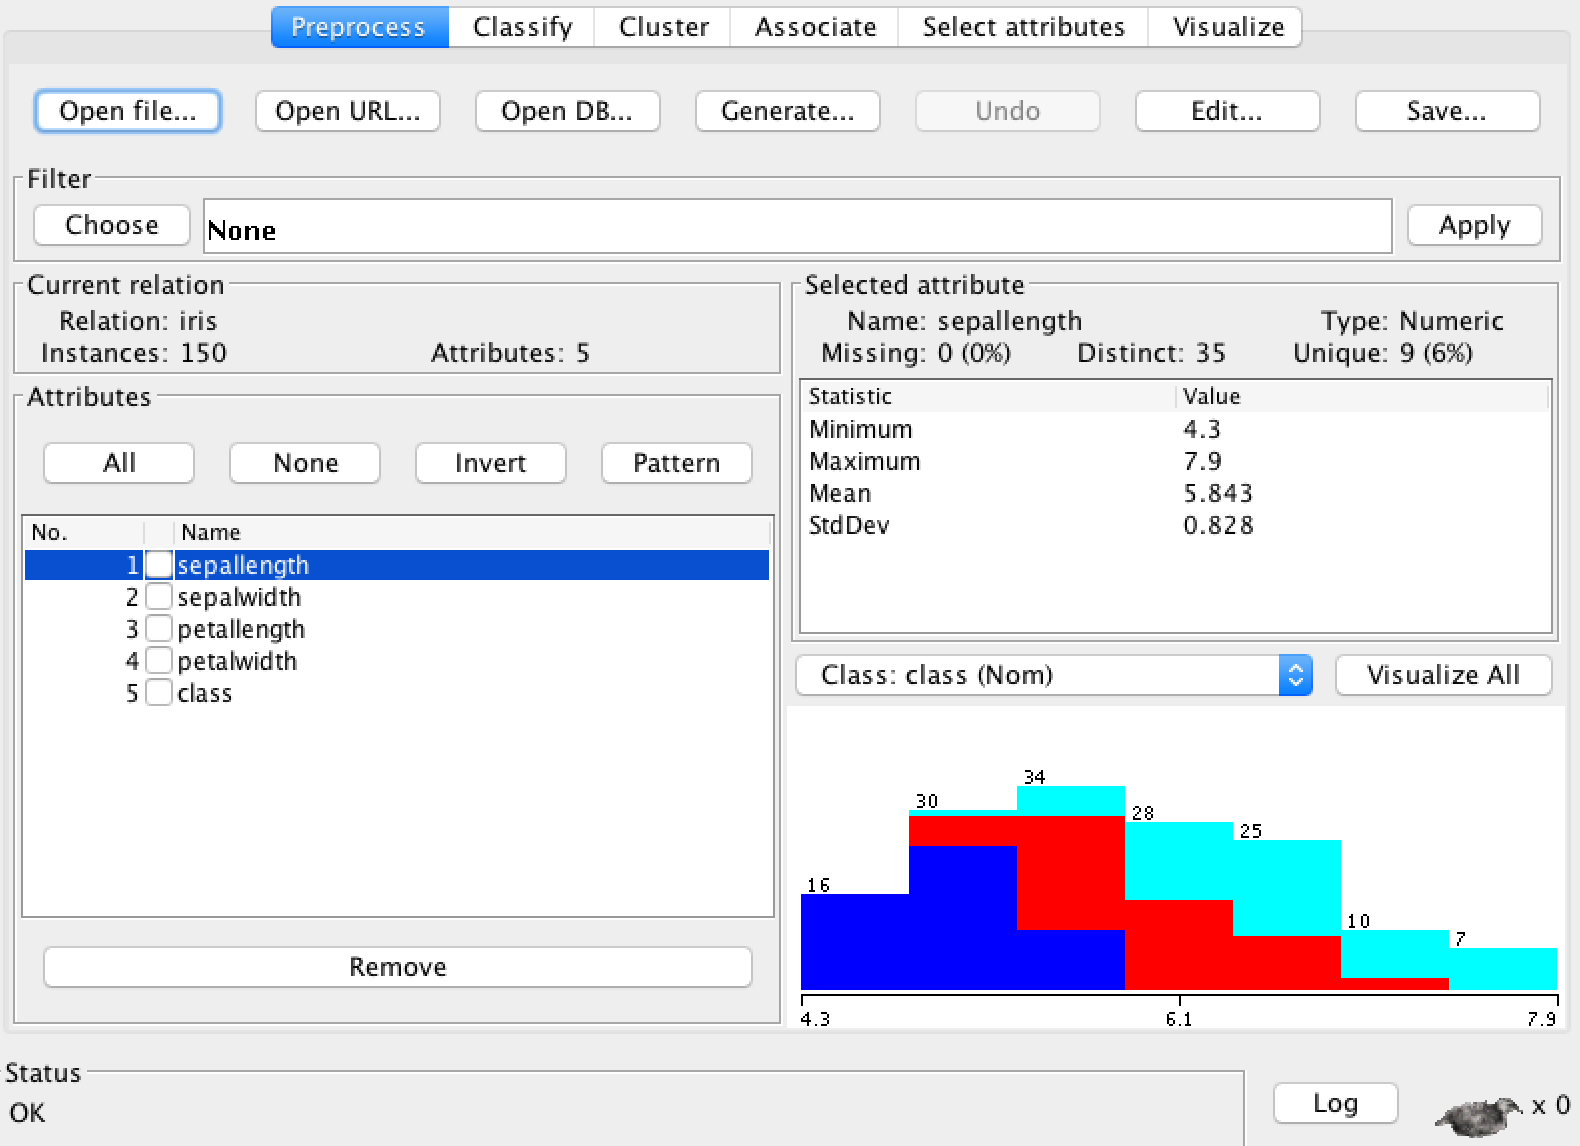
\includegraphics[width=0.5\textwidth]{wekaVisForIrisDataset.png}
 \caption{OneVsOne on a Multiclass Classification Data Set}
 \label{fig: original}
 \end{figure}

 \begin{figure}
 \centering
  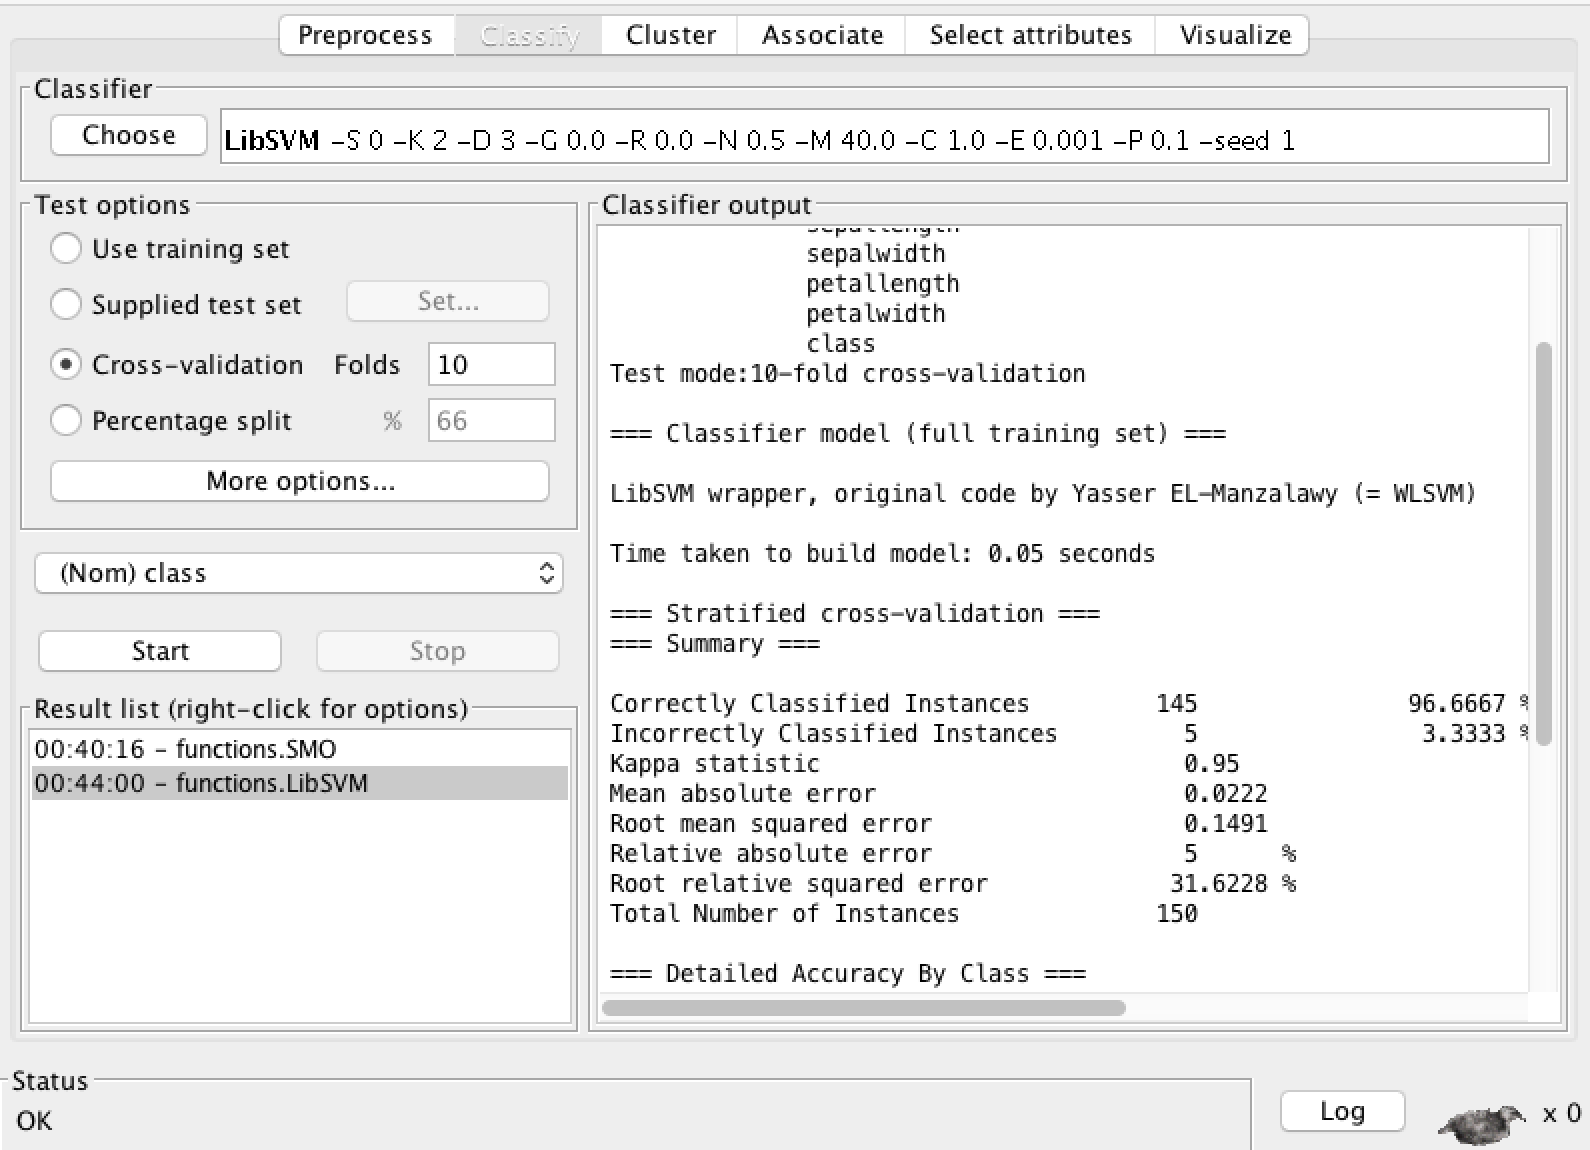
\includegraphics[width=0.5\textwidth]{wekaOneVsAllResult.png}
 \caption{Result of OneVsAllResult}
 \label{fig: onevsall}
 \end{figure}


The Sequential Minimal Optimization (SMO) implements a one vs one multi class SVM classifier, while the LibSVM classifier implements a one vs all classifier.\\

I used Weka to test the effectiveness and efficiency of both methods on a multi-class dataset: Iris dataset (provided by weka). I used Weka because it is a popular application for classification tasks and I did not have to write the code to test both classifiers.\\

The Iris dataset (iris.arff) is as follows:\\

@RELATION iris\\

{@ATTRIBUTE sepallength  REAL}\\
@ATTRIBUTE sepalwidth   REAL\\
@ATTRIBUTE petallength  REAL\\
@ATTRIBUTE petalwidth REAL\\
@ATTRIBUTE class  {Iris-setosa,Iris-versicolor,Iris-virginica}\\

There are 3 classes for classifying Iris flower based on the attributes: sepallength, sepalwidth, petallength and petalwidth. This is seen in Figure \ref{fig: original}\\

Figure \ref{fig: onevsone} shows the result of the One vs One (SMO) classification result\\

Figure \ref{fig: onevsall} shows the result of the One vs All (SMO) classification result
\begin{verbatim}

One vs One (SMO) classification result      One vs All (LibSVM) classification result

Time taken to build model: 0.12 seconds     Time taken to build model: 0.05 seconds


=== Stratified cross-validation ===        === Stratified cross-validation ===                                  
=== Summary ===                            === Summary ===

Correctly Classified Instances  144  96 % Correctly Classified Instances  144 96 %    
Incorrectly Classified Instances 6   4 %  Incorrectly Classified Instances  6  4 %
Kappa statistic                  0.94     Kappa statistic            0.94  
Mean absolute error              0.2311   Mean absolute error        0.2311
Root mean squared error          0.288    Root mean squared error    0.288 
Relative absolute error          52%      Relative absolute error    52  %
Root relative squared error      61.101%  Root relative squared error 61.101%
Total Number of Instances        150      Total Number of Instances   150     

\end{verbatim}

Both methods show the same accuracy (96\%). This is because they implement the same underlying SVM algorithm. SVMs are inherently used for binary classification, but can be used for multi-class problems using:
\begin{enumerate}
\item One vs rest (one vs all)
\item One vs One (multiple classifiers; choose the class that is selected by the most classifiers)
\end{enumerate}
However, the one-vs-one method is less efficient since it requires multiple sub-classification tasks: this is seen in the faster processing time of the LIBSVM method. 




\end{homeworkProblem}
%----------------------------------------------------------------------------------------
% PROBLEM 5
%----------------------------------------------------------------------------------------

\begin{homeworkProblem}

Use K-means and spherical K-means to cluster the data points in Exercise
9.9. How do the clusterings differ?\\

\textbf{Solution 5:}\\

\lstinputlisting[caption=K-means and spherical K-means Clustering Code Snippet, language=python]{9.9.py}

The k-means clustering algorithm attempts to minimize a Euclidean distance between the center of a given cluster and the members of the cluster.\\ 
I used sklearn's k-means algorithm to cluster the data point. This is demonstrated with \textit{testKMeans()} in listing 2\\


I specified 3 clusters for the algorithm.
Figure \ref{fig: SphKcluster} shows the clustering result. This is  exactly the same as the hierarchical clustering result.\\


\textbf{Spherical k-means}\\

Spherical k-means attempts to minimize the angle between the center of a given cluster and the members of the cluster.\\

I used a python library (spherecluster) to test spherical k-means. The result was different from the previous k-means and hierarchical clustering. I believe this is because it minimizes angles and not just distances. Figure \ref{fig:kcluster} shows the result of the spherical k-means clustering.

\begin{figure}
 \centering
  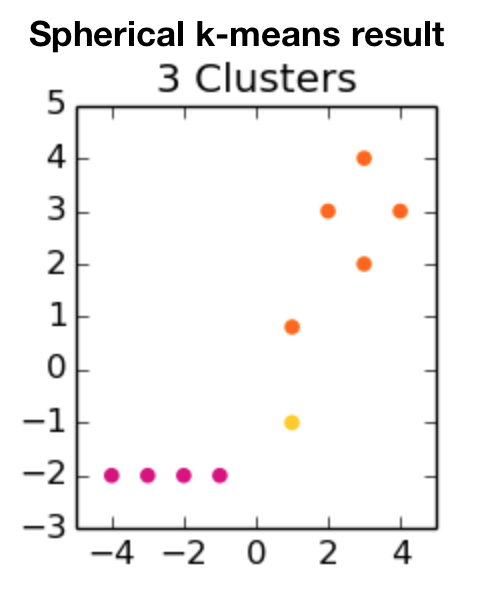
\includegraphics[width=0.5\textwidth]{spericalKmeansClustResult.png}
 \caption{Spherical K-clustering}
 \label{fig:SphKcluster}
 \end{figure}



 \begin{figure}
 \centering
  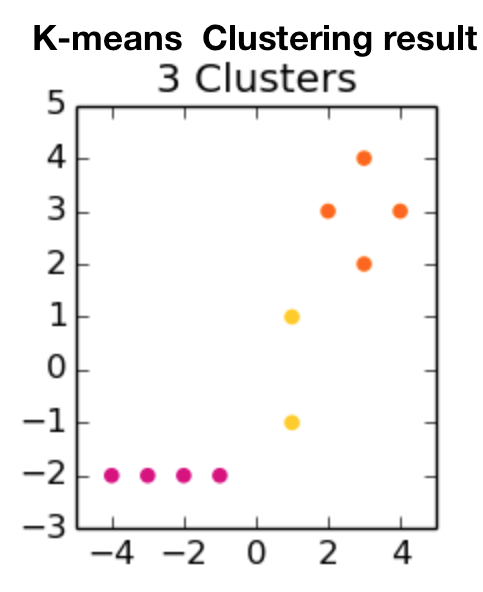
\includegraphics[width=0.5\textwidth]{kmeansClustResult.png}
 \caption{Kmeans Clustering}
 \label{fig:kcluster}
 \end{figure}





\end{homeworkProblem}
%----------------------------------------------------------------------------------------
% PROBLEM 6
%----------------------------------------------------------------------------------------

\begin{homeworkProblem}

\lstinputlisting[caption=Multiple-Bernoulli and Multinomial Models Code Snippet, language=python]{9.4.py}

9.4. For some classification data set, compute estimates for P(w|c) for all words
using both the multiple-Bernoulli and multinomial models. Compare the multipleBernoulli
estimates with the multinomial estimates. How do they differ? Do the
estimates diverge more for certain types of terms?

\textbf{Solution}\\

\textbf{Multiple-Bernoulli Model}\\

The goal of multiple-Bernoulli model is to estimate the probability that a term is belongs to a class. In this event space, a document is represented as a binary metrix. The rows are the docoments and the columns are the  vocabulary. The entries are binary, 1 if a term occurs in the document or 0 if it doesn't occur.\\

In order to compute estimates for p(w|c) for all words using multiple-bernoulli model, I used a youtube classification data set to learn if a word is spam and not spam. This data set is saved in \textit{Youtube02-KatyPerry.csv}  I calculated the probability of a random word belonging to this classifier using the maxumum likelihood estimate which is :\\
P(w|c) = $\frac{dfw,c}{Nc}$. This is demontrated with \textit{calcMultBernoulli(w, c, trainingSet)} in Listing 3.\\

\textbf{Youtube Data Snippet}\\

\begin{verbatim}

Content               Class
I really like this song. <> 0
my son love so much <> 0
Y LOVE YOU <> 0
follow me on instagram bigboss286 <> 1
why the elephant have a broken horn <> 0
Free itunes $25 giftcard codes: http://shhort.com/a?r=OOCnjqU2b <> 1
Where did she find all that make up in a freakin jungle?! <> 0
so cute that monkey *-*!  <> 0
Nice song <> 0
subscribe please  <> 1
\end{verbatim}

\textbf{Multinomial Model}\\

Multinomial is a generalization of multiple-bernoulli. This model takes into consideration the importance term frequence feature has in retrieval and classification. The goal of this model is to estimate the probability that a term occurs in a document. This model helps to determine the weight of a document since it considers the number of times each word occurs in the document.\\

In order to compute the probability that a term belongs to a class, I used the maximum likelihood estimate for the multinomial model: P(w|c) = $\frac{tf_w,_c}{|c|}$. This is demonstrated in \textit{calcMultinomial(w, c, trainingSet)} in Listing 3. I used both distributions to compute estimate for words.\\

\begin{verbatim}

Multiple-Bernoulli
  song
    P(SPAM) =  0.05714285714285714
    P(NOT) =  0.21142857142857144

Multinomial
    P(SPAM) =  0.0034982508745627187
    P(NOT) =  0.019770114942528734


Multiple-Bernoulli
  buy
    P(SPAM) =  0.005714285714285714
    P(NOT) =  0.0

Multinomial
    P(SPAM) =  0.0002498750624687656
    P(NOT) =  0.0



Multiple-Bernoulli
  world
    P(SPAM) =  0.017142857142857144
    P(NOT) =  0.03428571428571429

Multinomial
    P(SPAM) =  0.0007496251874062968
    P(NOT) =  0.002758620689655172


 Multiple-Bernoulli
  video
    P(SPAM) =  0.10857142857142857
    P(NOT) =  0.14285714285714285

Multinomial
    P(SPAM) =  0.004747626186906547
    P(NOT) =  0.012413793103448275
                                              
\end{verbatim}

According to Multiple-Bernoulli, the probability that the word ``buy'' is SPAM is 0.005714285714285714 and the probability that it is NOT SPAM is 0.0. Since the probability of SPAM is higher, the term ``buy'' is SPAM.\\

According to Multinomial the probability that the word ``buy'' is SPAM is 0.0002498750624687656 and the probability that it is NOT SPAM is 0.0. Since the probability of SPAM is higher, the term ``buy'' is  SPAM\\

According to Multiple-Bernoulli, the probability that the word ``song'' is SPAM is 0.05714285714285714 and the probability that it is NOT SPAM is 0.21142857142857144. Since the probability of NOT SPAM is higher, the term ``song'' is NOT SPAM.\\

According to Multinomial the probability that the word ``song'' is SPAM is 0.0034982508745627187 and the probability that it is NOT SPAM is 0.019770114942528734. Since the probability of NOT SPAM is higher, the term ``song'' is NOT SPAM\\

From my observation according to my out in \textit{proOutput.txt}, Multiple-Bernoulli gives the term more weight because it has a higher probabiity. Although Multinomial differentiates a term from SPAM and NOT SPAM correctly, the weight is not high. Multiple-bernoulli is more confident because of the weight. This applies to all output result. I think this is the reseaon why the text \textit{Search Engines Information Retrieval} states that multiple-bernoulli is good at estimating short documents, and my data set consists of short documents




\end{homeworkProblem}
%----------------------------------------------------------------------------------------
% PROBLEM 7
%----------------------------------------------------------------------------------------

\begin{homeworkProblem}


8.5. Generate the mean average precision, recall-precision graph, average NDCG
at 5 and 10, and precision at 10 for the entire CACM query set.\\

\textbf{Solution}\\
\lstinputlisting[caption=Mean Average Precision Code Snippet, language=python]{8.5.py}


In order to compute the mean average precision, recall-precision graph, average NDCG at 5 and 10, and precision at 10 for the entire CACM query set, I took the following steps:\\

For Mean Average Precision, I used ranking window of size 10 in the CACM query set. This is demonsrated with \textit{calcAvgPrecForQuery(query, K, data):} in Listing 4.\\

Mean Average Precision: 0.719438244048\\


For recall-precision graph, I used \textit{genPrecRecallGraph(query, K, data)} in Listing 4 to generate the recall-precision graph after computing recall-precision with \textit{calcPrecRecallAtK(query, K, data, returnType='single')} Figure \ref{fig:rprec10} is the recall- precision graph at 10 and Figure \ref{fig:rprec5} is the recall- precision graph at 5. \\

For average NDCG at 5 and 10, I used \textit{ndcg\_at\_k(ranking5, 5)} and \textit{ndcg\_at\_k(ranking10, 10)} to compute NDCG at 5 and NDCG at 10 and calculated the average of NDCG at 5 and 10 respectively. The result is in \textit{map-prec-at-10-avg-ndcg-r-prect.txt}. This file also contains result of precision at 10 for all CACM query set.\\

The result snippet for precion at 10 for all CACM query set and average NDCG is given below:

\begin{verbatim}
  query: 1
  Precision at 10: 0.5
  average NDCG: 1.0

query: 2
  Precision at 10: 0.3
  average NDCG: 1.0

query: 3
  Precision at 10: 0.6
  average NDCG: 1.0

query: 4
  Precision at 10: 1.0
  average NDCG: 1.0

query: 5
  Precision at 10: 0.8
  average NDCG: 1.0

\end{verbatim}

Average NDCG for all CACM query set is 1.0.\\

For Precision at 10 for the entire CACM query set, I used \textit{(calcPrecRecallAtK(query, 10, lines)['precision'])} in Listing 4 to calculate precicion at 10 for the entire CACM query set and the result is in \textit{map-prec-at-10-avg-ndcg-r-prect.txt}.


\begin{figure}
 \centering
  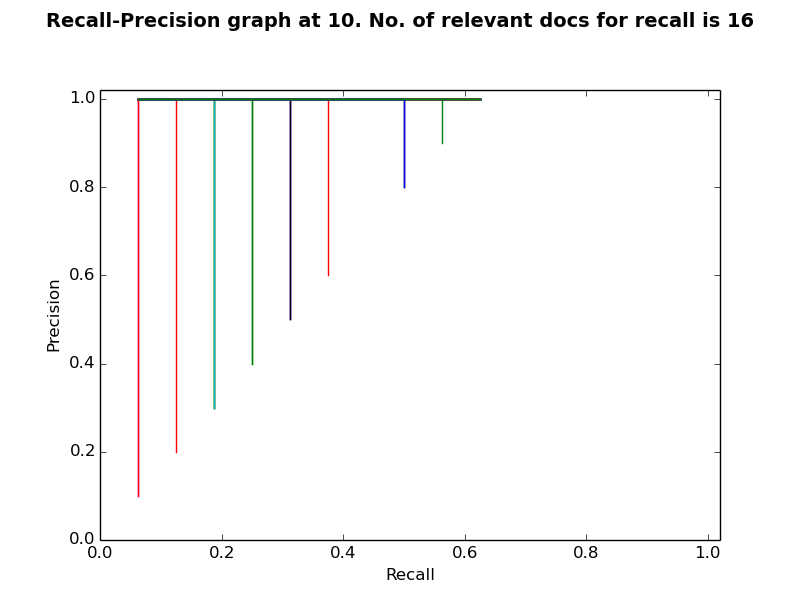
\includegraphics[width=0.5\textwidth]{recall-precision-at-10.png}
 \caption{Recall-Precision at 10}
 \label{fig:rprec10}
 \end{figure}



 \begin{figure}
 \centering
  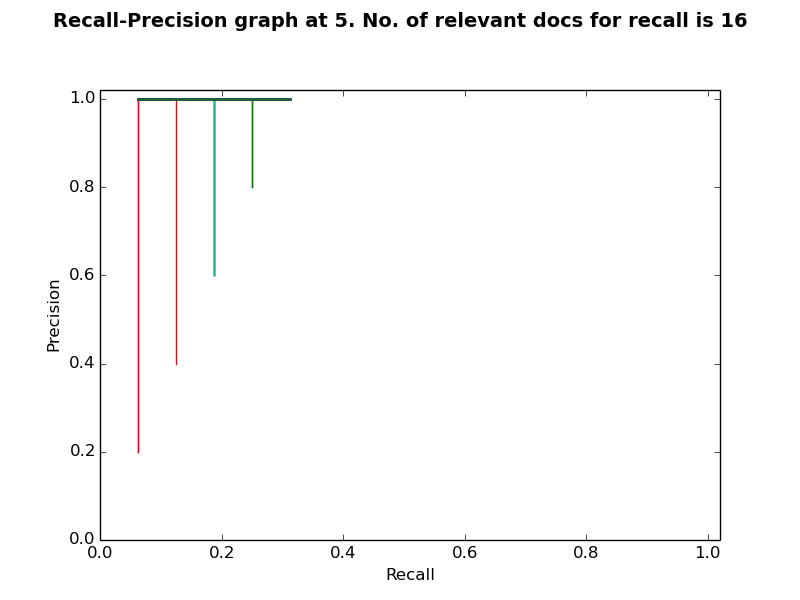
\includegraphics[width=0.5\textwidth]{recall-precision-at-5.png}
 \caption{Recall-Precision at 5}
 \label{fig:rprec5}
 \end{figure}

\end{homeworkProblem}
%----------------------------------------------------------------------------------------
% PROBLEM 8
%----------------------------------------------------------------------------------------

\begin{homeworkProblem}

8.7. Another measure that has been used in a number of evaluations is R-precision.
This is defined as the precision at R documents, where R is the number of relevant
documents for a query. It is used in situations where there is a large variation in
the number of relevant documents per query. Calculate the average R-precision
for the CACM query set and compare it to the other measures.\\

\textbf{Solution}\\
R-precision is the at R-documents, R is the number of relevant documents to a query. In order to compute R-precision for the CACM quert set, 
I used \textit{r\_precision(r)} in Listing 4\\

MAP: 0.719438244048\\
R-Precision: 0.8125

According to the result output, R-precision is highly correlated with the Mean Average Precision.

\end{homeworkProblem}

\nocite{*}
\bibliographystyle{plain}
\bibliography{A4Ref}

\end{document}
